\documentclass[12pt, letterpaper]{article}
\usepackage{graphicx} %LaTeX package to import graphics
\graphicspath{{images/}} %configuring the graphicx package

\title{My first LaTex documnet}
\author{Hubert Farnsworth\thanks{Funded by the Overleaf team.}}
\date{February 2022}
\begin{document}
\maketitle
We have now added a title, author and date to our first \LaTeX{} document!
% First document. This is a simple example, with no 
% extra parameters or packages included. Now I have 
% added more text and need to recompile the document.
\parindent0pt% To remove the paragraph indentation

Some of the \textbf{greatest}
discoveries in \underline{science} 
were made by \textbf{\textit{accident}}.

Some of the greatest \emph{discoveries} in science 
were made by accident.

\textit{Some of the greatest \emph{discoveries} 
in science were made by accident.}

\textbf{Some of the greatest \emph{discoveries} 
in science were made by accident.}

The universe is immense and it seems to be homogeneous, 
on a large scale, everywhere we look.

% The \includegraphcs command is 
% provided (implemented) by the 
% graphicx package
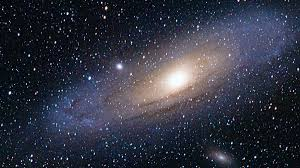
\includegraphics{universe}  
 
There's a picture of a galaxy above.

\begin{itemize}
    \item The individual entries are indicated with a black dot, a so-called bullet.
    \item The text in the entries may be of any length.
\end{itemize}

\begin{figure}[h]
    \centering
    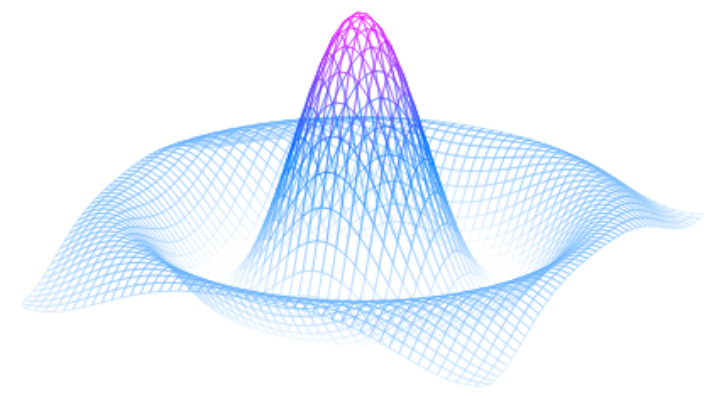
\includegraphics[width=0.75\textwidth]{mesh}
    \caption{A nice plot.}
    \label{fig:mesh1}
\end{figure}
 
As you can see in figure \ref{fig:mesh1}, the function grows near the origin. This example is on page \pageref{fig:mesh1}.

\begin{enumerate}
    \item This is the first entry in our list.
    \item The list numbers increase with each entry we add.
\end{enumerate}

In physics, the mass-energy equivalence is stated 
by the equation $E=mc^2$, discovered in 1905 by Albert Einstein.

\begin{math}
    E=mc^2
\end{math} is typeset in a paragraph using inline math mode---as is $E=mc^2$, and so too is \(E=mc^2\).

The mass-energy equivalence is described by the famous equation
\[ E=mc^2 \] discovered in 1905 by Albert Einstein. 

In natural units ($c = 1$), the formula expresses the identity
\begin{equation}
E=m
\end{equation}



\end{document}